%!TEX root = ./nips_2018_sketchmcmc_supp.tex

\section{Details of Computing $(F_{\theta_{n}^*\#\hat{\mu}}^{-1} \circ F_{\theta^*_{n}\#\nu}) $}


\umut{Antoine. -- sorting, interpolation etc}

\begin{figure}
\begin{centering}
\setlength\tabcolsep{1pt}
\begin{tabular}{cccccc}
$\lambda=0$ & $\lambda=0.1$ & $\lambda=0.2$ & $\lambda=0.3$ & $\lambda=0.5$ & $\lambda=1$\tabularnewline
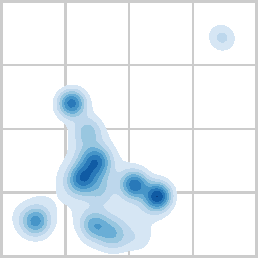
\includegraphics[width=2cm]{figures/supplementary/regularization/r0_output_dist_k=70-crop.pdf} & 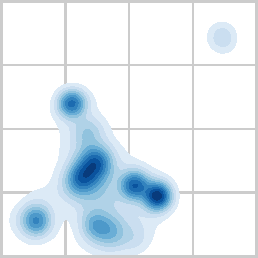
\includegraphics[width=2cm]{figures/supplementary/regularization/r01_output_dist_k=70-crop.pdf} & 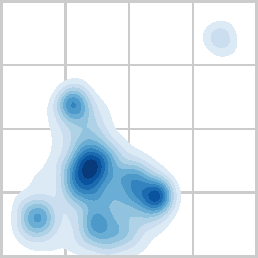
\includegraphics[width=2cm]{figures/supplementary/regularization/r02_output_dist_k=70-crop.pdf} &  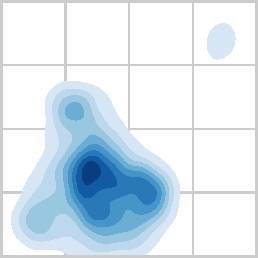
\includegraphics[width=2cm]{figures/supplementary/regularization/r03_output_dist_k=70-crop.pdf}&  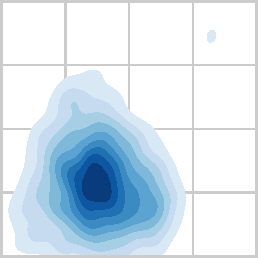
\includegraphics[width=2cm]{figures/supplementary/regularization/r05_output_dist_k=70-crop.pdf} &  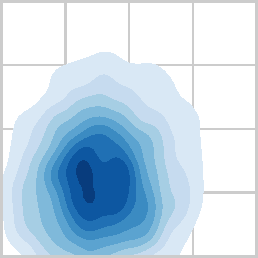
\includegraphics[width=2cm]{figures/supplementary/regularization/r1_output_dist_k=70-crop.pdf}
\end{tabular}
\par\end{centering}
\caption{Influence of the regularization parameter $\lambda$. The higher $\lambda$, the more entropic the output distribution.\label{fig:lambda_supp}}
\end{figure}
